\documentclass[11pt,a4paper]{article}

% ==== Pacotes (união dos preâmbulos dos Relatórios 2 e 3) ====
\usepackage[T1]{fontenc}
\usepackage[utf8]{inputenc}
\usepackage[brazil]{babel}
\usepackage{lmodern}
\usepackage[a4paper,margin=2.2cm]{geometry}
\usepackage{setspace}
\usepackage{booktabs}
\usepackage{array}
\usepackage{hyperref}
\usepackage{graphicx}
\usepackage{float}
\usepackage{placeins}
\usepackage{indentfirst}
\usepackage{enumitem}
\usepackage{longtable}
\usepackage{amsmath}
\usepackage{subcaption}
\usepackage{titlesec}

\setstretch{1.05}

\hypersetup{
    colorlinks=true,
    linkcolor=black,
    urlcolor=blue,
    citecolor=black
}

\title{
\textbf{Relatório Técnico Final de Ciência de Dados} \\[4pt]
\large Da Predição Clínica à Vigilância Socioambiental: um Sistema Integrado de
Análise e Previsão da Esquistossomose no Brasil
}

\author{
Luiz Gabriel Correia dos Santos (15639682) \\
Ana Paula de Abreu Batista (12688424) \\
Italo Carlos Martins Bresciani (15461782)
}

\date{\today}

\begin{document}

\maketitle

\begin{abstract}
Este relatório final consolida todas as etapas do \textit{Projeto Caramujo}, um sistema de vigilância
computacional para a esquistossomose no Brasil. O trabalho evoluiu em três fases complementares. Na
\textbf{Fase I}, conduziu-se uma Análise Exploratória de Dados (EDA) sobre os registros do SINAN
(extraídos via \texttt{PySUS}), acompanhada de análises temporais e geoespaciais e de uma tentativa de
predição supervisionada de desfechos clínicos (Cura, Não Cura, Óbito). As limitações dessa abordagem
--- ausência de variáveis clínicas densas e forte desbalanceamento --- motivaram a \textbf{Fase II}, na
qual o problema foi reformulado: em vez de prever o desfecho individual, passou-se a prever o
\emph{risco municipal}, integrando dados epidemiológicos (SINAN), ambientais (MapBiomas), censitários
(IBGE) e de saneamento (SNIS). Empregou-se \textit{K-Means} para descobrir cinco perfis de risco e
\textit{Random Forest} com \textit{Undersampling} para prever a vulnerabilidade a partir exclusivamente
da infraestrutura e da geografia, com validação \textit{Out-of-Time} (2015--2025). Por fim, a
\textbf{Fase III} materializou todos os achados em uma aplicação interativa em \textit{Streamlit},
transformando a pesquisa em uma ferramenta operacional de saúde pública. Os resultados comprovam que a
assinatura socioambiental de contágio (pequenos açudes e esgotamento sanitário) possui alto sinal
preditivo e é estruturalmente atemporal, além de documentar a retração histórica da doença no território
nacional.
\end{abstract}

\tableofcontents
\bigskip
\hrule

% ===================================================================
\part{Fase I --- Análise Exploratória e Predição de Desfechos Clínicos}
% ===================================================================

\section{Introdução}

A esquistossomose é uma doença parasitária crônica considerada um importante problema de saúde pública no
Brasil, especialmente em regiões com infraestrutura sanitária precária e exposição frequente a coleções
hídricas contaminadas.

O Sistema de Informação de Agravos de Notificação (SINAN) disponibiliza registros epidemiológicos em
larga escala, permitindo investigações analíticas sobre distribuição espacial, dinâmica temporal e
fatores associados aos desfechos clínicos da doença.

Nesta primeira fase, buscou-se responder à seguinte pergunta:

\begin{quote}
É possível, a partir do perfil epidemiológico e clínico de um caso notificado, construir um modelo capaz
de predizer seu desfecho?
\end{quote}

Para isso, esta etapa foi dividida em três frentes:

\begin{enumerate}
    \item Análise Exploratória de Dados (EDA);
    \item Análise Geoespacial e Temporal;
    \item Aprendizado Supervisionado para predição de desfechos.
\end{enumerate}

\section{Base de Dados}

Os dados utilizados foram obtidos via biblioteca \texttt{PySUS}, utilizando registros do SINAN referentes
ao agravo de esquistossomose (\texttt{ESQU}).

Após carregamento e concatenação das bases anuais, foram aplicados filtros de qualificação para construção
da base analítica.

\subsection{Filtros Aplicados}

\begin{itemize}
    \item Casos positivos no exame Hoffman (\texttt{AN\_QUANT == 1});
    \item Remoção de desfechos ignorados;
    \item Exclusão de óbitos por causas não relacionadas à esquistossomose;
    \item Padronização de variáveis temporais e categóricas.
\end{itemize}

As classes finais utilizadas na modelagem foram:

\begin{itemize}
    \item 1 = Cura;
    \item 2 = Não Cura;
    \item 3 = Óbito por esquistossomose.
\end{itemize}

\section{Metodologia}

\subsection{Pré-processamento}

As seguintes etapas de tratamento foram realizadas:

\begin{itemize}
    \item Conversão de strings vazias para \texttt{NaN};
    \item Conversão de datas epidemiológicas;
    \item Padronização de códigos IBGE;
    \item Criação de variáveis derivadas temporais;
    \item Conversão de variáveis categóricas;
    \item Filtragem de inconsistências temporais.
\end{itemize}

\subsection{Análise Exploratória}

A EDA foi conduzida com os seguintes objetivos:

\begin{enumerate}
    \item Avaliar completude e consistência dos registros;
    \item Identificar padrões temporais;
    \item Analisar concentração geográfica;
    \item Caracterizar o perfil demográfico dos pacientes;
    \item Investigar padrões clínicos e terapêuticos.
\end{enumerate}

\subsection{Análise Geoespacial}

Foram realizadas análises espaciais focadas principalmente nos estados de Minas Gerais e Espírito Santo,
identificados como áreas prioritárias devido à alta incidência média histórica.

A análise buscou identificar:

\begin{itemize}
    \item Municípios com maior concentração de casos;
    \item Relação entre distribuição espacial e hidrografia;
    \item Influência de fatores socioambientais;
    \item Possíveis focos locais de transmissão.
\end{itemize}

\subsection{Aprendizado Supervisionado}

O problema foi formulado como uma tarefa de classificação multiclasse supervisionada.

Os modelos baseline avaliados foram:

\begin{itemize}
    \item Regressão Logística;
    \item XGBoost;
    \item Versões com e sem PCA.
\end{itemize}

A estratégia de avaliação priorizou:

\begin{itemize}
    \item Recall para classes críticas;
    \item F1-macro;
    \item Precision;
    \item Comparação entre trade-offs clínicos.
\end{itemize}

\section{Resultados da Fase Clínica}

\subsection{Tendência Temporal}

Observou-se uma redução significativa no número de casos notificados entre 2007 e 2025, embora com
oscilações relevantes em determinados períodos.

\begin{figure}[H]
\centering
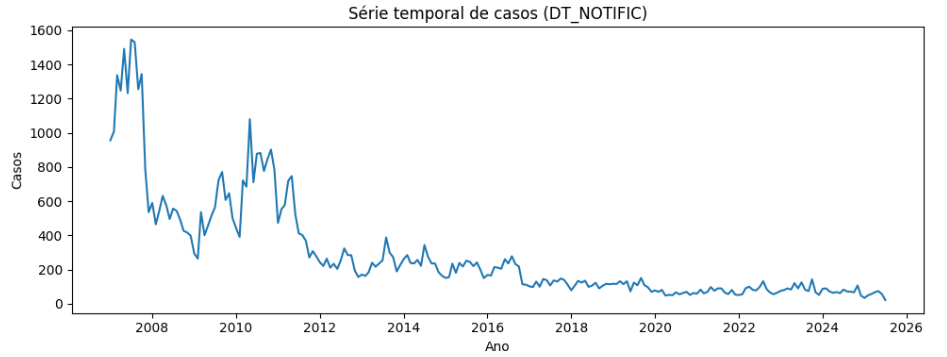
\includegraphics[width=\textwidth]{temporal.png}
\caption{Tendência temporal de casos de esquistossomose.}
\end{figure}

Os resultados sugerem avanços no controle da doença, possivelmente relacionados à ampliação do saneamento
básico e melhorias em estratégias de vigilância epidemiológica.

\subsection{Distribuição Geográfica}

Minas Gerais e Espírito Santo apresentaram as maiores incidências médias por 100 mil habitantes no período
analisado.

\begin{figure}[H]
\centering
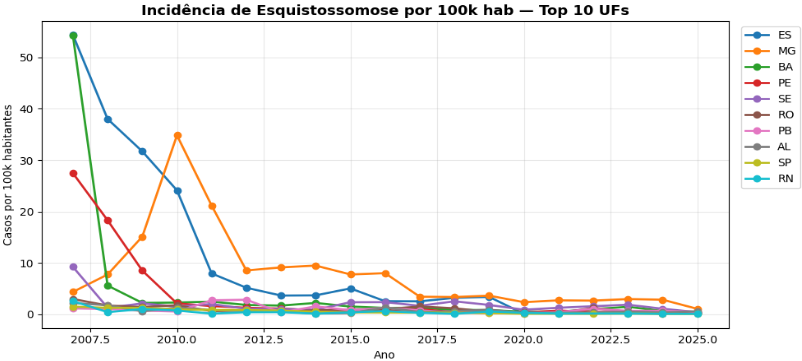
\includegraphics[width=\textwidth]{incidencia.png}
\caption{Incidência média por UF.}
\end{figure}

A concentração dos casos nesses estados motivou análises geoespaciais mais aprofundadas.

\subsection{Focos Municipais}

Foi realizada uma análise visual comparando a distribuição espacial dos municípios com maior concentração
de casos e a presença da bacia do Rio São Francisco. Os resultados não indicaram relação espacial evidente
entre os principais focos de notificação e a proximidade com a bacia hidrográfica principal da região.

Esse resultado sugere que a dinâmica de transmissão da esquistossomose pode estar mais associada a fatores
locais do que à presença dos grandes cursos d'água. Entre os fatores potencialmente mais relevantes
destacam-se:

\begin{itemize}
    \item saneamento básico precário;
    \item coleções hídricas menores e áreas de água parada;
    \item presença do hospedeiro intermediário;
    \item condições socioeconômicas locais.
\end{itemize}

Dessa forma, embora não tenha sido observada associação visual relevante com a bacia do Rio São Francisco,
análises futuras podem incorporar outros corpos d'água regionais, como lagoas, açudes e pequenas coleções
hídricas --- exatamente o caminho aprofundado na Fase II deste projeto.

\subsection{Tempo de Encerramento}

A análise do tempo de encerramento dos casos mostrou diferenças relevantes entre os desfechos clínicos.

\begin{itemize}
    \item Casos de óbito apresentaram mediana extremamente baixa;
    \item Casos de cura concentraram-se em torno de 10 dias;
    \item Casos de não cura exibiram distribuição bimodal.
\end{itemize}

A variável \texttt{tempo\_encerramento\_dias} demonstrou forte potencial discriminativo entre os desfechos
analisados. Entretanto, essa variável deve ser interpretada com cautela em cenários preditivos, pois o
encerramento do caso ocorre temporalmente muito próximo do registro do desfecho clínico, podendo introduzir
vazamento de informação (\textit{data leakage}).

\subsection{Clusterização Clínica}

Foram realizadas tentativas exploratórias de clusterização com o objetivo de identificar possíveis
agrupamentos naturais entre os casos notificados. Entretanto, os resultados não produziram agrupamentos
clinicamente interpretáveis.

As principais limitações identificadas foram:

\begin{itemize}
    \item desbalanceamento entre features;
    \item alta cardinalidade de variáveis geográficas;
    \item ausência de informações clínicas detalhadas;
    \item forte dominância de atributos administrativos.
\end{itemize}

Dessa forma, concluiu-se que, para esta base específica, abordagens geoespaciais apresentaram maior
potencial analítico do que a clusterização puramente clínica --- percepção que direcionou toda a Fase II.

\section{Predição de Desfecho Clínico}

\subsection{Features Utilizadas}

\begin{longtable}{p{5cm}p{6cm}p{3cm}}
\toprule
\textbf{Atributo} & \textbf{Descrição} & \textbf{Tipo} \\
\midrule
CS\_SEXO & Sexo do paciente & Categórico \\
CS\_GESTANT & Gestante & Categórico \\
CS\_RACA & Raça/cor & Categórico \\
CS\_ESCOL\_N & Escolaridade & Ordinal \\
FORMA & Forma clínica & Categórico \\
TRATAM & Tratamento realizado & Categórico \\
SG\_UF & UF de residência & Geográfico \\
COUFINF & UF provável de infecção & Geográfico \\
delay\_notificacao\_dias & Sintomas até notificação & Numérico \\
tempo\_encerramento\_dias & Sintomas até encerramento & Numérico \\
IDADE\_PROCESSADA & Idade do paciente & Numérico \\
\bottomrule
\end{longtable}

\subsection{Resultados dos Modelos}

\begin{figure}[H]
\centering
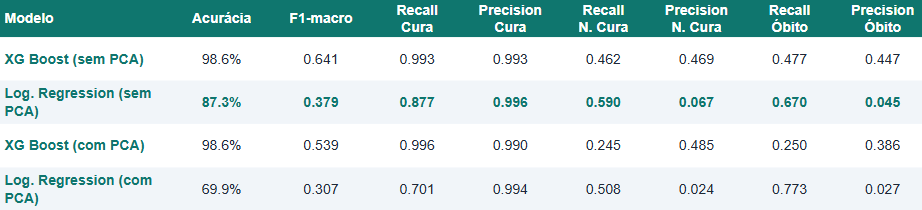
\includegraphics[width=\textwidth]{resultados.png}
\caption{Comparação entre modelos baseline.}
\end{figure}

\subsection{Discussão dos Resultados}

Os principais achados foram:

\begin{itemize}
    \item O uso de PCA prejudicou o desempenho de ambos os modelos baseline, indicando perda de informação
    relevante durante a redução de dimensionalidade;

    \item O XGBoost apresentou o melhor equilíbrio entre \textit{precision} e \textit{recall} nas classes
    críticas (Não Cura e Óbito), alcançando aproximadamente 45--46\% tanto em cobertura quanto em acerto
    dessas classes;

    \item A regressão logística apresentou elevado número de falsos positivos, refletido em valores muito
    baixos de \textit{precision} para as classes minoritárias (entre 2\% e 7\%);

    \item A forte dominância da classe majoritária (Cura) influenciou significativamente as métricas
    globais, resultando em valores superiores a 99\% de \textit{precision} para essa classe em todos os
    modelos avaliados;

    \item O principal desafio permaneceu a identificação confiável de casos graves. Assim, o modelo ideal
    deve priorizar elevado \textit{recall} para classes críticas sem comprometer excessivamente a
    \textit{precision}.
\end{itemize}

\subsection{Limitações da Fase Clínica}

As principais limitações desta etapa foram: alta ausência de dados clínicos; inconsistências temporais;
possível viés de subnotificação; alta cardinalidade de variáveis geográficas; e desbalanceamento entre
classes. Variáveis potencialmente relevantes para prognóstico clínico não estavam disponíveis na base
pública utilizada. Tais restrições motivaram a mudança de paradigma detalhada na Fase II.

% ===================================================================
\part{Fase II --- Integração Socioambiental e Perfis de Risco}
% ===================================================================

\section{Reformulação do Problema}

Para superar as limitações dos dados puramente clínicos e o desbalanceamento das classes de desfecho, a
abordagem metodológica foi reestruturada. A nova pergunta norteadora passou a ser:

\begin{quote}
\textbf{Quais características estruturais e ambientais fazem uma cidade se tornar um polo de transmissão da
esquistossomose, e é possível prever esse risco?}
\end{quote}

Para responder a essa questão, superamos a análise univariada e integramos dados do Ministério da Saúde,
IBGE, MapBiomas e SNIS, modelando a dinâmica complexa entre população, água parada e saneamento.

\section{Base de Dados e Engenharia de Atributos}

Para capturar o padrão dinâmico da saúde pública, o escopo de dados foi ampliado e as seguintes bases foram
concatenadas utilizando o período de referência inicial de \textbf{2011 a 2014} para treinamento:

\begin{itemize}
    \item \textbf{Saúde (SINAN via PySUS):} Notificações confirmadas por exame de fezes positivo
    (\texttt{AN\_QUALI = 1}).
    \item \textbf{População (IBGE):} Dados populacionais anuais, utilizados para nivelar a comparação entre
    municípios através do cálculo de \textit{Incidência por 100 mil habitantes}.
    \item \textbf{Geografia e Hidrografia (MapBiomas):} Foi aplicada uma engenharia de atributos crucial.
    Como grandes hidrelétricas e áreas de mineração não transmitem a doença (devido à profundidade e
    dinâmica da água), criou-se a métrica \texttt{açudes\_canais\_ha}. Esta variável isola a "água pequena"
    (açudes rurais e canais de irrigação), verdadeiro habitat do caramujo vetor.
    \item \textbf{Saneamento (SNIS):} Taxa de coleta de esgoto doméstico. Para lidar com valores faltantes,
    aplicou-se um \textit{pipeline} avançado de imputação: primeiro temporal (a cidade corrige seus anos
    faltantes baseada em seu histórico) e, em seguida, geoespacial (herança da mediana estadual/nacional do
    ano).
\end{itemize}

\section{Metodologia Socioambiental}

\subsection{Agrupamento de Perfis de Risco (Aprendizado Não Supervisionado)}
Para evitar distorções estatísticas, a base foi filtrada para conter apenas os municípios com ao menos um
caso positivo no período. Utilizou-se o algoritmo \textbf{K-Means}, validado pelos métodos do Cotovelo e da
Silhueta, determinando o número ideal de $K=5$ grupos (\textit{clusters}). O agrupamento avaliou
simultaneamente incidência, população, área de açudes e taxa de esgoto, identificando automaticamente a
assinatura do "Alto Risco".

\subsection{Modelagem Preditiva (Aprendizado Supervisionado)}
Após a clusterização, os rótulos gerados foram utilizados como alvo (\textit{target}) para um algoritmo
\textbf{Random Forest}. O modelo foi "cego" em relação aos dados de saúde (incidência e casos) e treinado
exclusivamente com variáveis ambientais e de infraestrutura. Devido ao forte desbalanceamento (poucas
cidades de alto risco), a base foi dividida em treino e teste (70/30 estratificado) e aplicou-se a técnica
de \textbf{Undersampling} (proporção 1:2) apenas sobre a base de treino, forçando o modelo a aprender as
diferenças estatísticas vitais sem adotar uma postura estática.

\subsection{Validação Temporal (Out-of-Time)}
Para testar o fenômeno do \textit{Concept Drift} (mudança de comportamento do mundo real no futuro), o
modelo treinado nos dados de 2011--2014 foi desafiado a classificar o risco de municípios em duas janelas
do "futuro": \textbf{2015--2019} e \textbf{2020--2025}.

\section{Resultados e Discussão Socioambiental}

\subsection{Os 5 Perfis da Esquistossomose no Brasil}
O \textit{K-Means} conseguiu isolar com clareza as dinâmicas demográficas e sanitárias do país:

\begin{enumerate}
    \item \textbf{Grandes Metrópoles (Cluster 3):} Populações milionárias (ex: SP e RJ), incidência nula. O
    algoritmo isolou os \textit{outliers} demográficos para não distorcer a análise.
    \item \textbf{Centros Médios com Grandes Represas (Cluster 4):} Confirma o paradoxo hídrico: maior área
    de água antrópica do país, porém incidência muito baixa (4,02/100k), provando que o caramujo não
    prolifera nessas condições.
    \item \textbf{Centros Urbanos Estruturados (Cluster 0):} Cidades de médio porte com boa cobertura de
    esgoto (76\%) e controle epidemiológico.
    \item \textbf{Cinturão de Vulnerabilidade (Cluster 1):} Menor cobertura de esgoto (31,5\%). Funciona
    como um risco latente; a incidência é moderada, mas o ambiente está propício a surtos.
    \item \textbf{Epicentro da Doença --- Alto Risco Absoluto (Cluster 2):} Cidades muito pequenas, com
    forte contato humano com açudes periféricos e taxa de esgoto de gabinete mediana (62,9\%). Onde a
    incidência explodiu para impressionantes \textbf{778,02 casos por 100 mil habitantes}.
\end{enumerate}

\begin{table}[H]
    \centering
    \caption{Perfil médio das variáveis estruturais e epidemiológicas para cada grupo (cluster)
    identificado.}
    \label{tab:perfil_clusters}
    \renewcommand{\arraystretch}{1.2}
    \resizebox{\textwidth}{!}{%
    \begin{tabular}{@{}lcccc@{}}
        \toprule
        \textbf{Perfil (Cluster)} & \textbf{Incidência} & \textbf{Açudes/Canais} & \textbf{Taxa de Esgoto} & \textbf{População} \\
        & \textbf{(por 100k hab.)} & \textbf{(Hectares)} & \textbf{Média (\%)} & \textbf{Média} \\
        \midrule
        0 - Centros Estruturados & 19,94 & 41,02 & 76,34 & 99.484 \\
        1 - Cinturão de Vulnerabilidade & 11,30 & 61,70 & 31,57 & 68.008 \\
        2 - Epicentro (Alto Risco) & 778,02 & 3,44 & 62,97 & 11.101 \\
        3 - Grandes Metrópoles & 0,36 & 150,67 & 68,39 & 9.005.051 \\
        4 - Centros com Represas & 4,02 & 1.219,80 & 47,95 & 146.357 \\
        \bottomrule
    \end{tabular}%
    }
\end{table}

\begin{figure}[H]
    \centering
    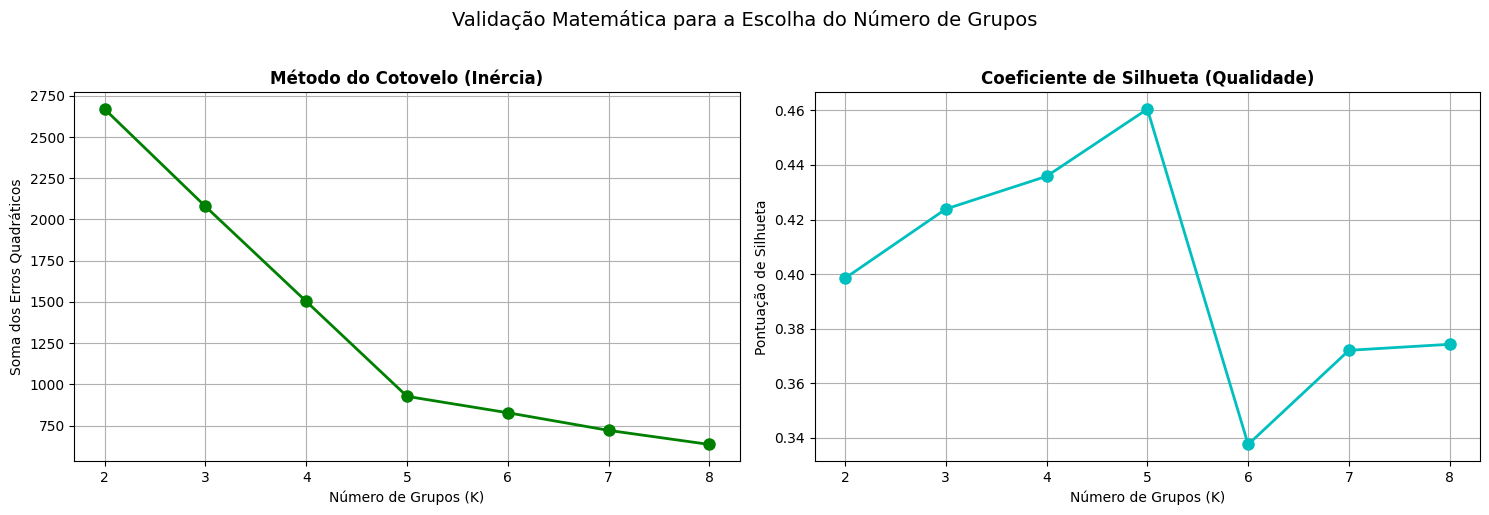
\includegraphics[width=0.9\textwidth]{cotovelo.png}
    \caption{Gráficos de validação matemática (Cotovelo e Silhueta) para a escolha do número de clusters.}
    \label{fig:cotovelo_clusters}
\end{figure}

\begin{figure}[H]
    \centering
    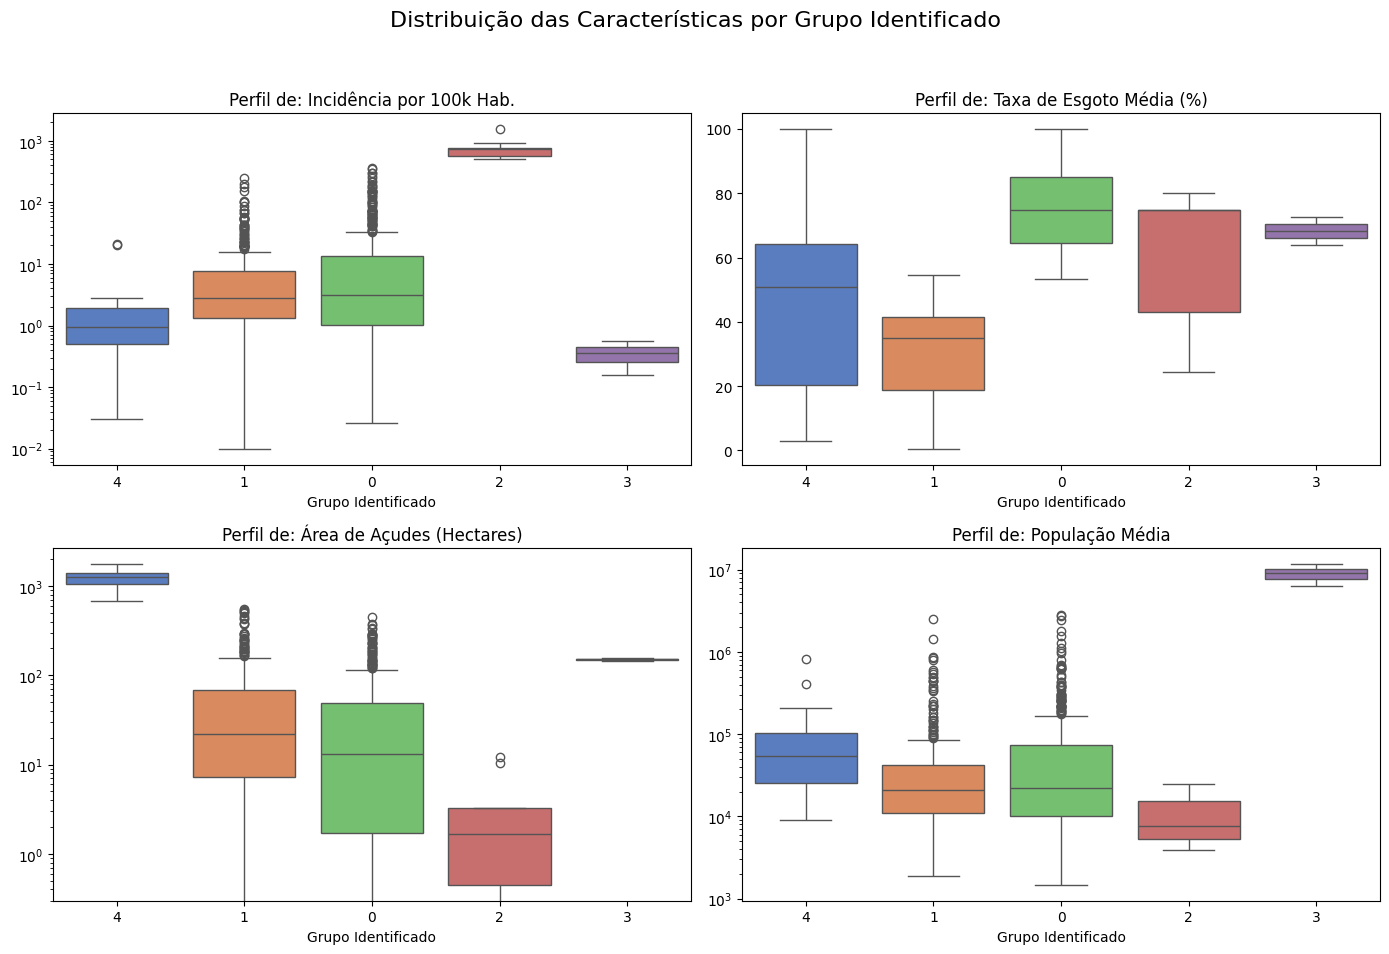
\includegraphics[width=0.9\textwidth]{boxplots.png}
    \caption{Boxplots das características estruturais e epidemiológicas por cluster.}
    \label{fig:boxplots_clusters}
\end{figure}

\subsection{A Importância das Variáveis}
A floresta aleatória balanceada revelou que as variáveis \texttt{açudes\_canais\_ha} (27,30\% de
importância) e \texttt{taxa\_esgoto\_media} (26,42\%) assumiram o protagonismo. A geografia natural
(\texttt{natural\_ha}) ficou em terceiro (21,55\%).

\begin{figure}[H]
    \centering
    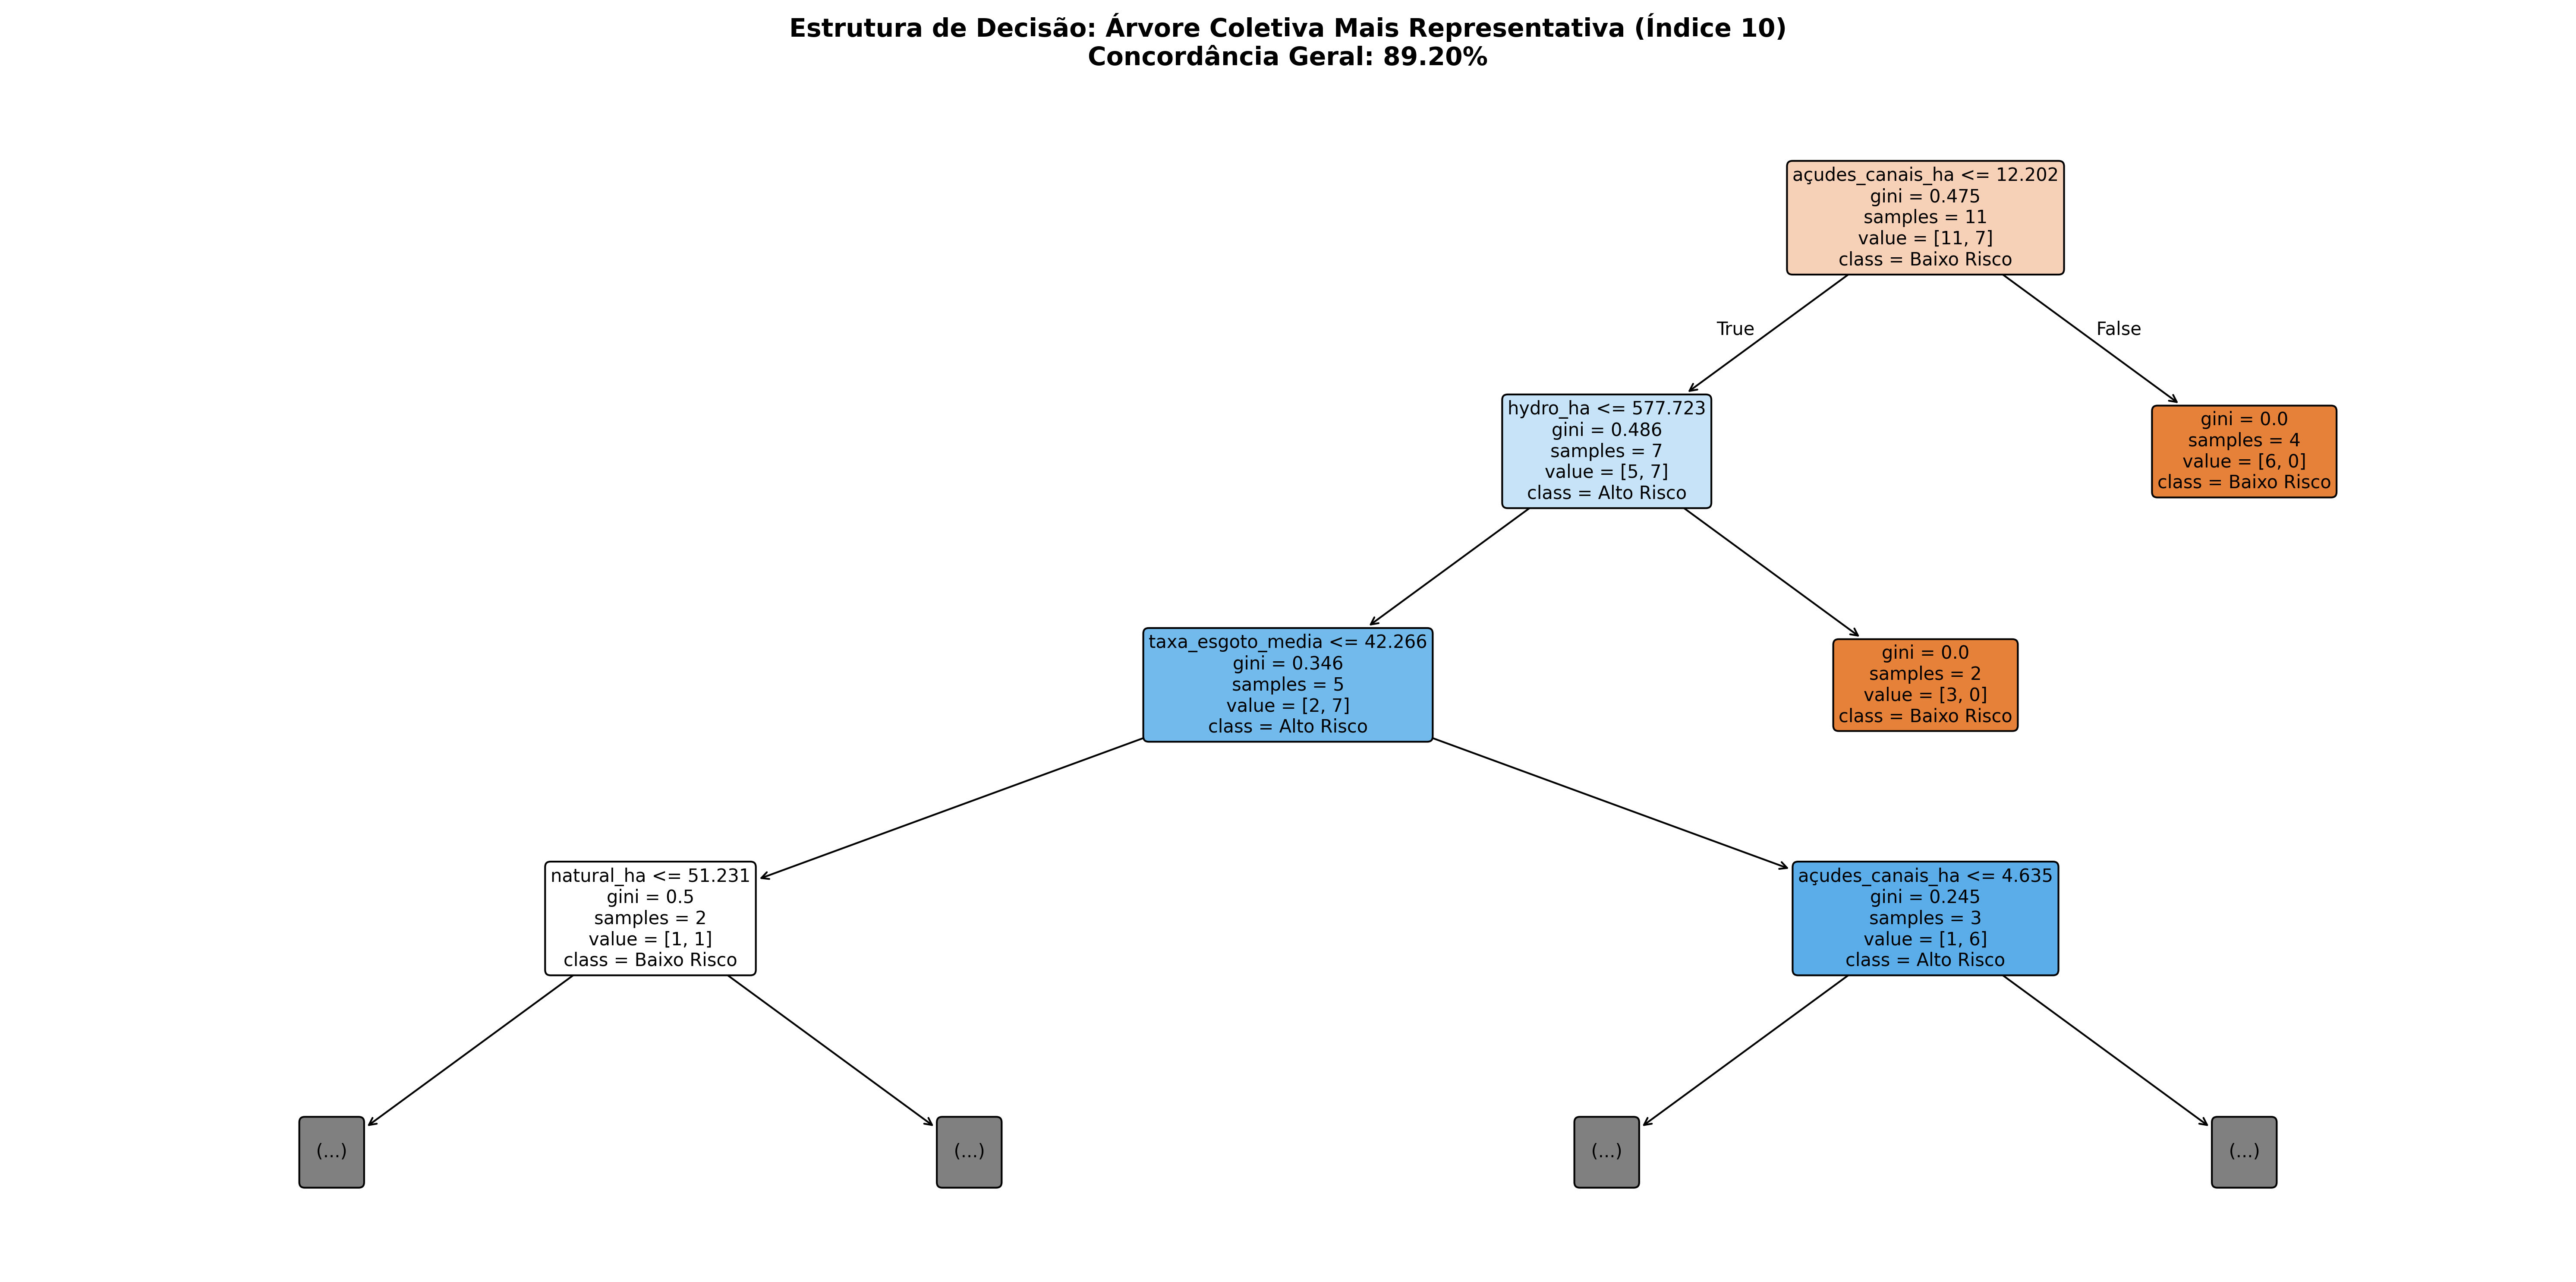
\includegraphics[width=0.9\textwidth]{arvore.png}
    \caption{Árvore mais representativa encontrada no Random Forest.}
    \label{fig:arvore}
\end{figure}

A modelagem evidenciou uma limitação crítica nos indicadores oficiais de infraestrutura. Municípios
endêmicos em Minas Gerais, a exemplo de Dom Silvério, registram 100\% de cobertura de esgotamento
sanitário no SNIS. Em abordagens preditivas convencionais, esse índice gerava falsos negativos ao mascarar
a vulnerabilidade real. A análise demonstrou, contudo, que a coleta de esgoto concentrada nos centros
urbanos não interrompe o ciclo de transmissão quando as populações periféricas e rurais permanecem
expostas a redes de pequenos açudes antrópicos.

\subsection{Validação Temporal e a Retração Histórica}
O ecossistema da doença foi encurralado na última década. No treino (2011--2014) havia 9 municípios no polo
absoluto de risco; em 2015--2019 caiu para 6; e em 2020--2025 colapsou para apenas 1 município.

No teste \textit{Out-of-Time}, o modelo obteve:
\begin{itemize}
    \item \textbf{Acurácia Global Estável:} 82,26\% no teste original, cerca de 75\% no quinquênio seguinte
    e patamar semelhante na década atual, confirmando a validade estrutural das regras aprendidas.
    \item \textbf{Mapeamento Preventivo:} centenas de municípios foram sinalizados como "focos emergentes"
    (falsos positivos) --- cidades que carregam a assinatura ambiental de risco, mas que ainda não
    explodiram em surto.
\end{itemize}

\begin{figure}[H]
    \centering
    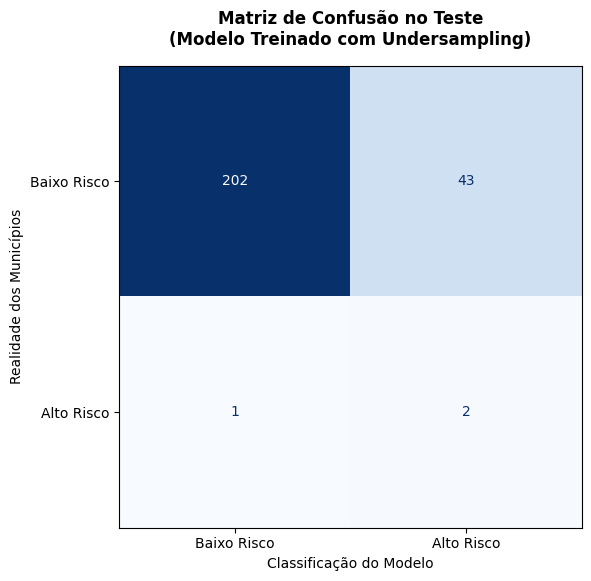
\includegraphics[width=0.5\textwidth]{matrizdeconfusao.png}
    \caption{Matriz de confusão do teste cego original (base 2011--2014).}
    \label{fig:matriz_orig}
\end{figure}

O modelo gerou dezenas de falsos positivos ao olhar para o futuro. Para a epidemiologia, isso atua como um
\textbf{mapa de vigilância ativa} (\textit{screening}). O modelo alertou que essas cidades continuam com o
ambiente perfeito para o parasita, e sua atual baixa incidência é mérito de intervenções de saúde,
mantendo a vulnerabilidade estrutural latente.

\begin{figure}[H]
    \centering
    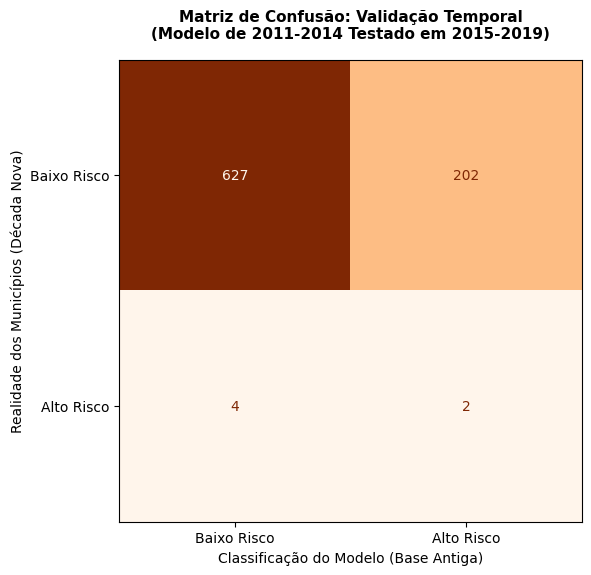
\includegraphics[width=0.49\textwidth]{2015-2019.png}
    \hfill
    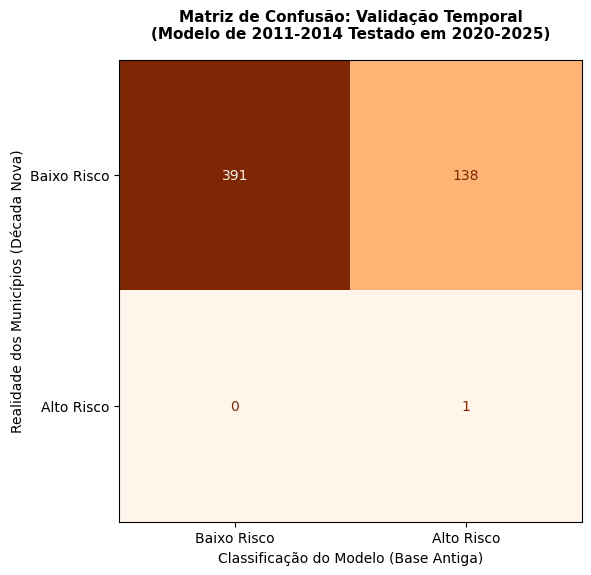
\includegraphics[width=0.49\textwidth]{2020-2025.png}
    \caption{Desempenho do modelo na validação temporal (\textit{Out-of-Time}). À esquerda, a aplicação em
    2015--2019 (202 falsos positivos preventivos); à direita, em 2020--2025 (138 alertas preventivos),
    evidenciando o extenso mapeamento de vulnerabilidade latente frente ao colapso do número de epicentros
    ativos.}
    \label{fig:matriz_temporal}
\end{figure}

% ===================================================================
\part{Fase III --- Sistema Interativo de Vigilância (Streamlit)}
% ===================================================================

\section{Da Pesquisa à Ferramenta Operacional}

Para que os achados das fases anteriores não permanecessem restritos a notebooks de análise, todo o
conhecimento foi consolidado em uma \textbf{aplicação web interativa} desenvolvida com o framework
\textit{Streamlit} (diretório \texttt{streamlit\_app/} do repositório). A aplicação traduz os modelos
matemáticos em uma interface de vigilância acessível a gestores e agentes de saúde pública, permitindo
explorar dados, perfis e previsões sem qualquer conhecimento de programação.

\subsection{Arquitetura da Aplicação}

A aplicação é organizada como um \textit{dashboard} de múltiplas páginas, com separação clara entre
apresentação e lógica de processamento:

\begin{itemize}
    \item \texttt{app.py} --- Página inicial de contextualização institucional do sistema.
    \item \texttt{pages/1\_Painel\_Epidemiologico.py} --- Painel descritivo do SINAN.
    \item \texttt{pages/2\_Mapeamento\_e\_Perfis.py} --- O Paradoxo do Saneamento e os 5 perfis do K-Means.
    \item \texttt{pages/3\_Aplicacao\_Temporal.py} --- Validação \textit{Out-of-Time} do modelo preditivo.
    \item \texttt{utils/data\_loader.py} --- Carregamento das bases (\texttt{.parquet} e \texttt{.csv}) com
    cache de memória (\texttt{@st.cache\_data}) para inicialização rápida.
    \item \texttt{utils/model\_trainer.py} --- Motor de \textit{Machine Learning}: treina o
    \textit{K-Means} e o \textit{Random Forest} em tempo de execução (com cache via
    \texttt{@st.cache\_resource}), reproduzindo \emph{fielmente} o \textit{pipeline} do notebook de
    modelagem (\textit{split} 70/30 estratificado e \textit{Undersampling} 1:2).
\end{itemize}

Um ponto central de engenharia é a \textbf{consistência com a pesquisa}: o modelo de referência é treinado
sobre a base histórica de 2011--2014 e reaplicado, sem reaprendizado, às janelas futuras. As matrizes de
confusão produzidas pela aplicação são \emph{numericamente idênticas} às reportadas na Fase II
(2015--2019: 202 alertas preventivos; 2020--2025: 138), garantindo rastreabilidade entre o relatório
científico e a ferramenta interativa.

\subsection{Página Inicial e Painel Epidemiológico}

A página inicial apresenta o propósito do sistema e orienta a navegação. O \textbf{Painel Epidemiológico}
(Figura~\ref{fig:st_painel}) oferece filtros dinâmicos por UF e por período, cartões de métricas
(total de casos confirmados, idade média, taxa de cura e municípios contaminados) e gráficos interativos
da série temporal e do perfil demográfico (idade, sexo, escolaridade e raça/cor).

\begin{figure}[H]
    \centering
    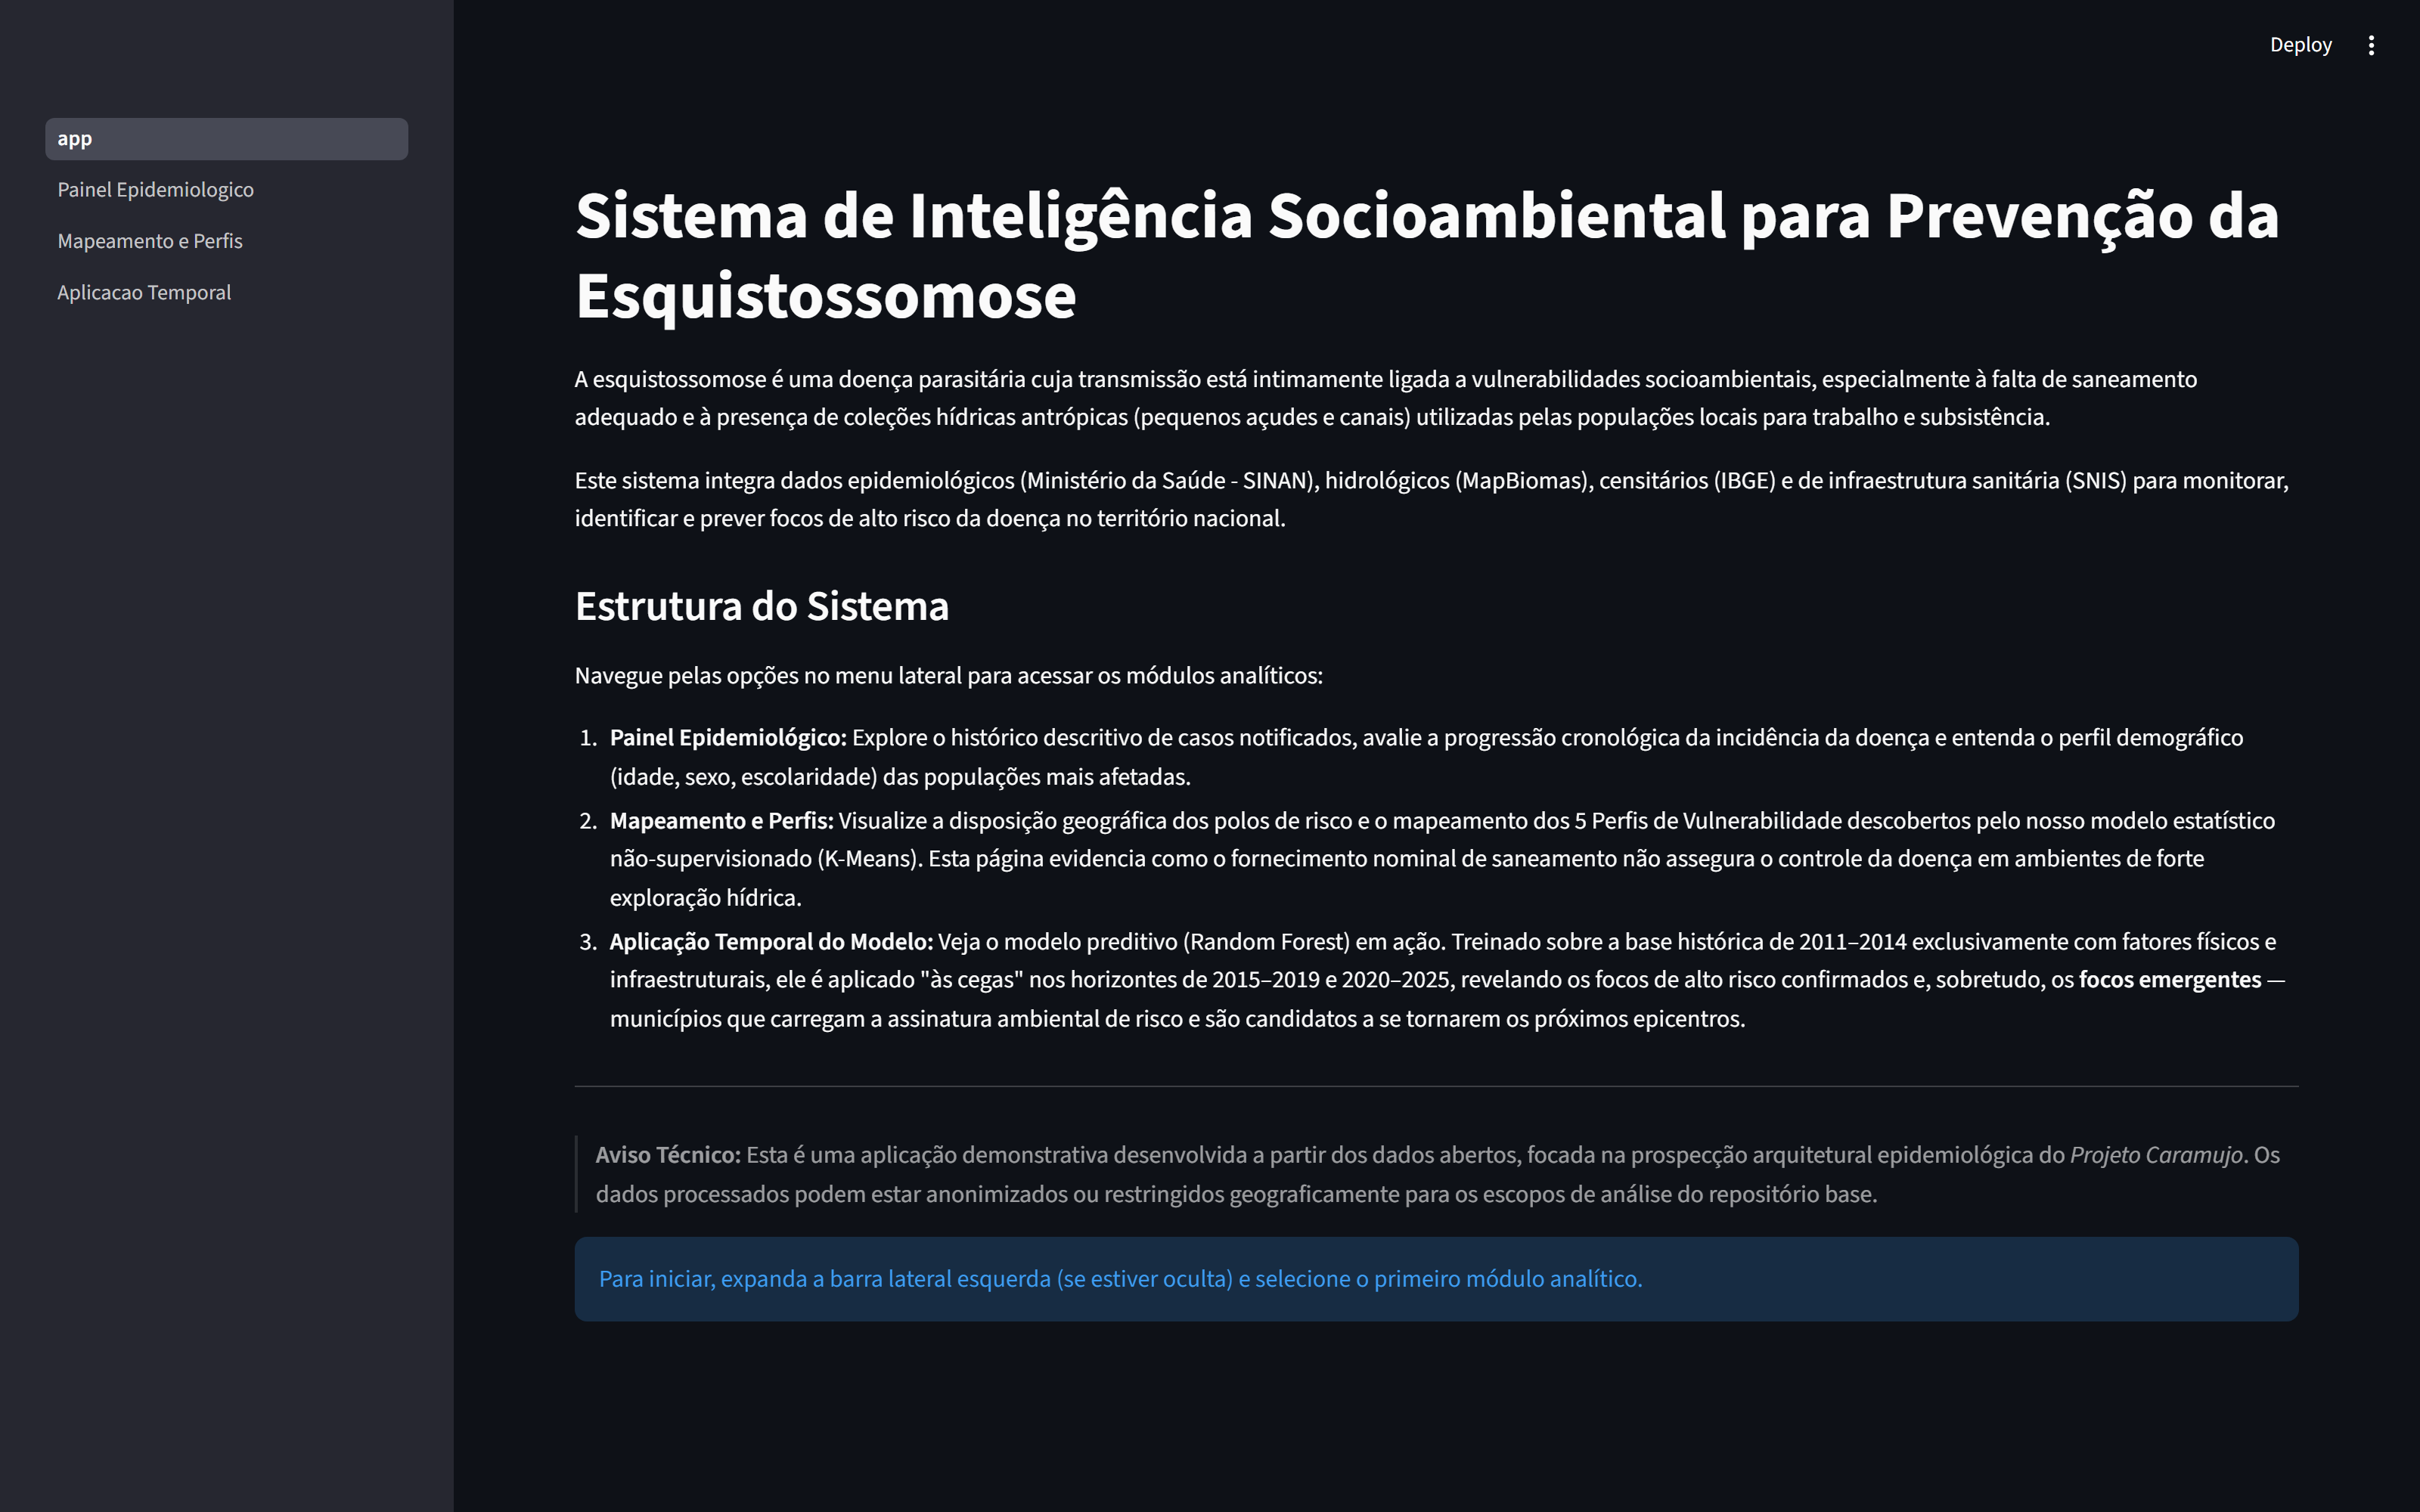
\includegraphics[width=\textwidth]{streamlit_home.png}
    \caption{Página inicial da aplicação: contextualização institucional do Projeto Caramujo.}
    \label{fig:st_home}
\end{figure}

\begin{figure}[H]
    \centering
    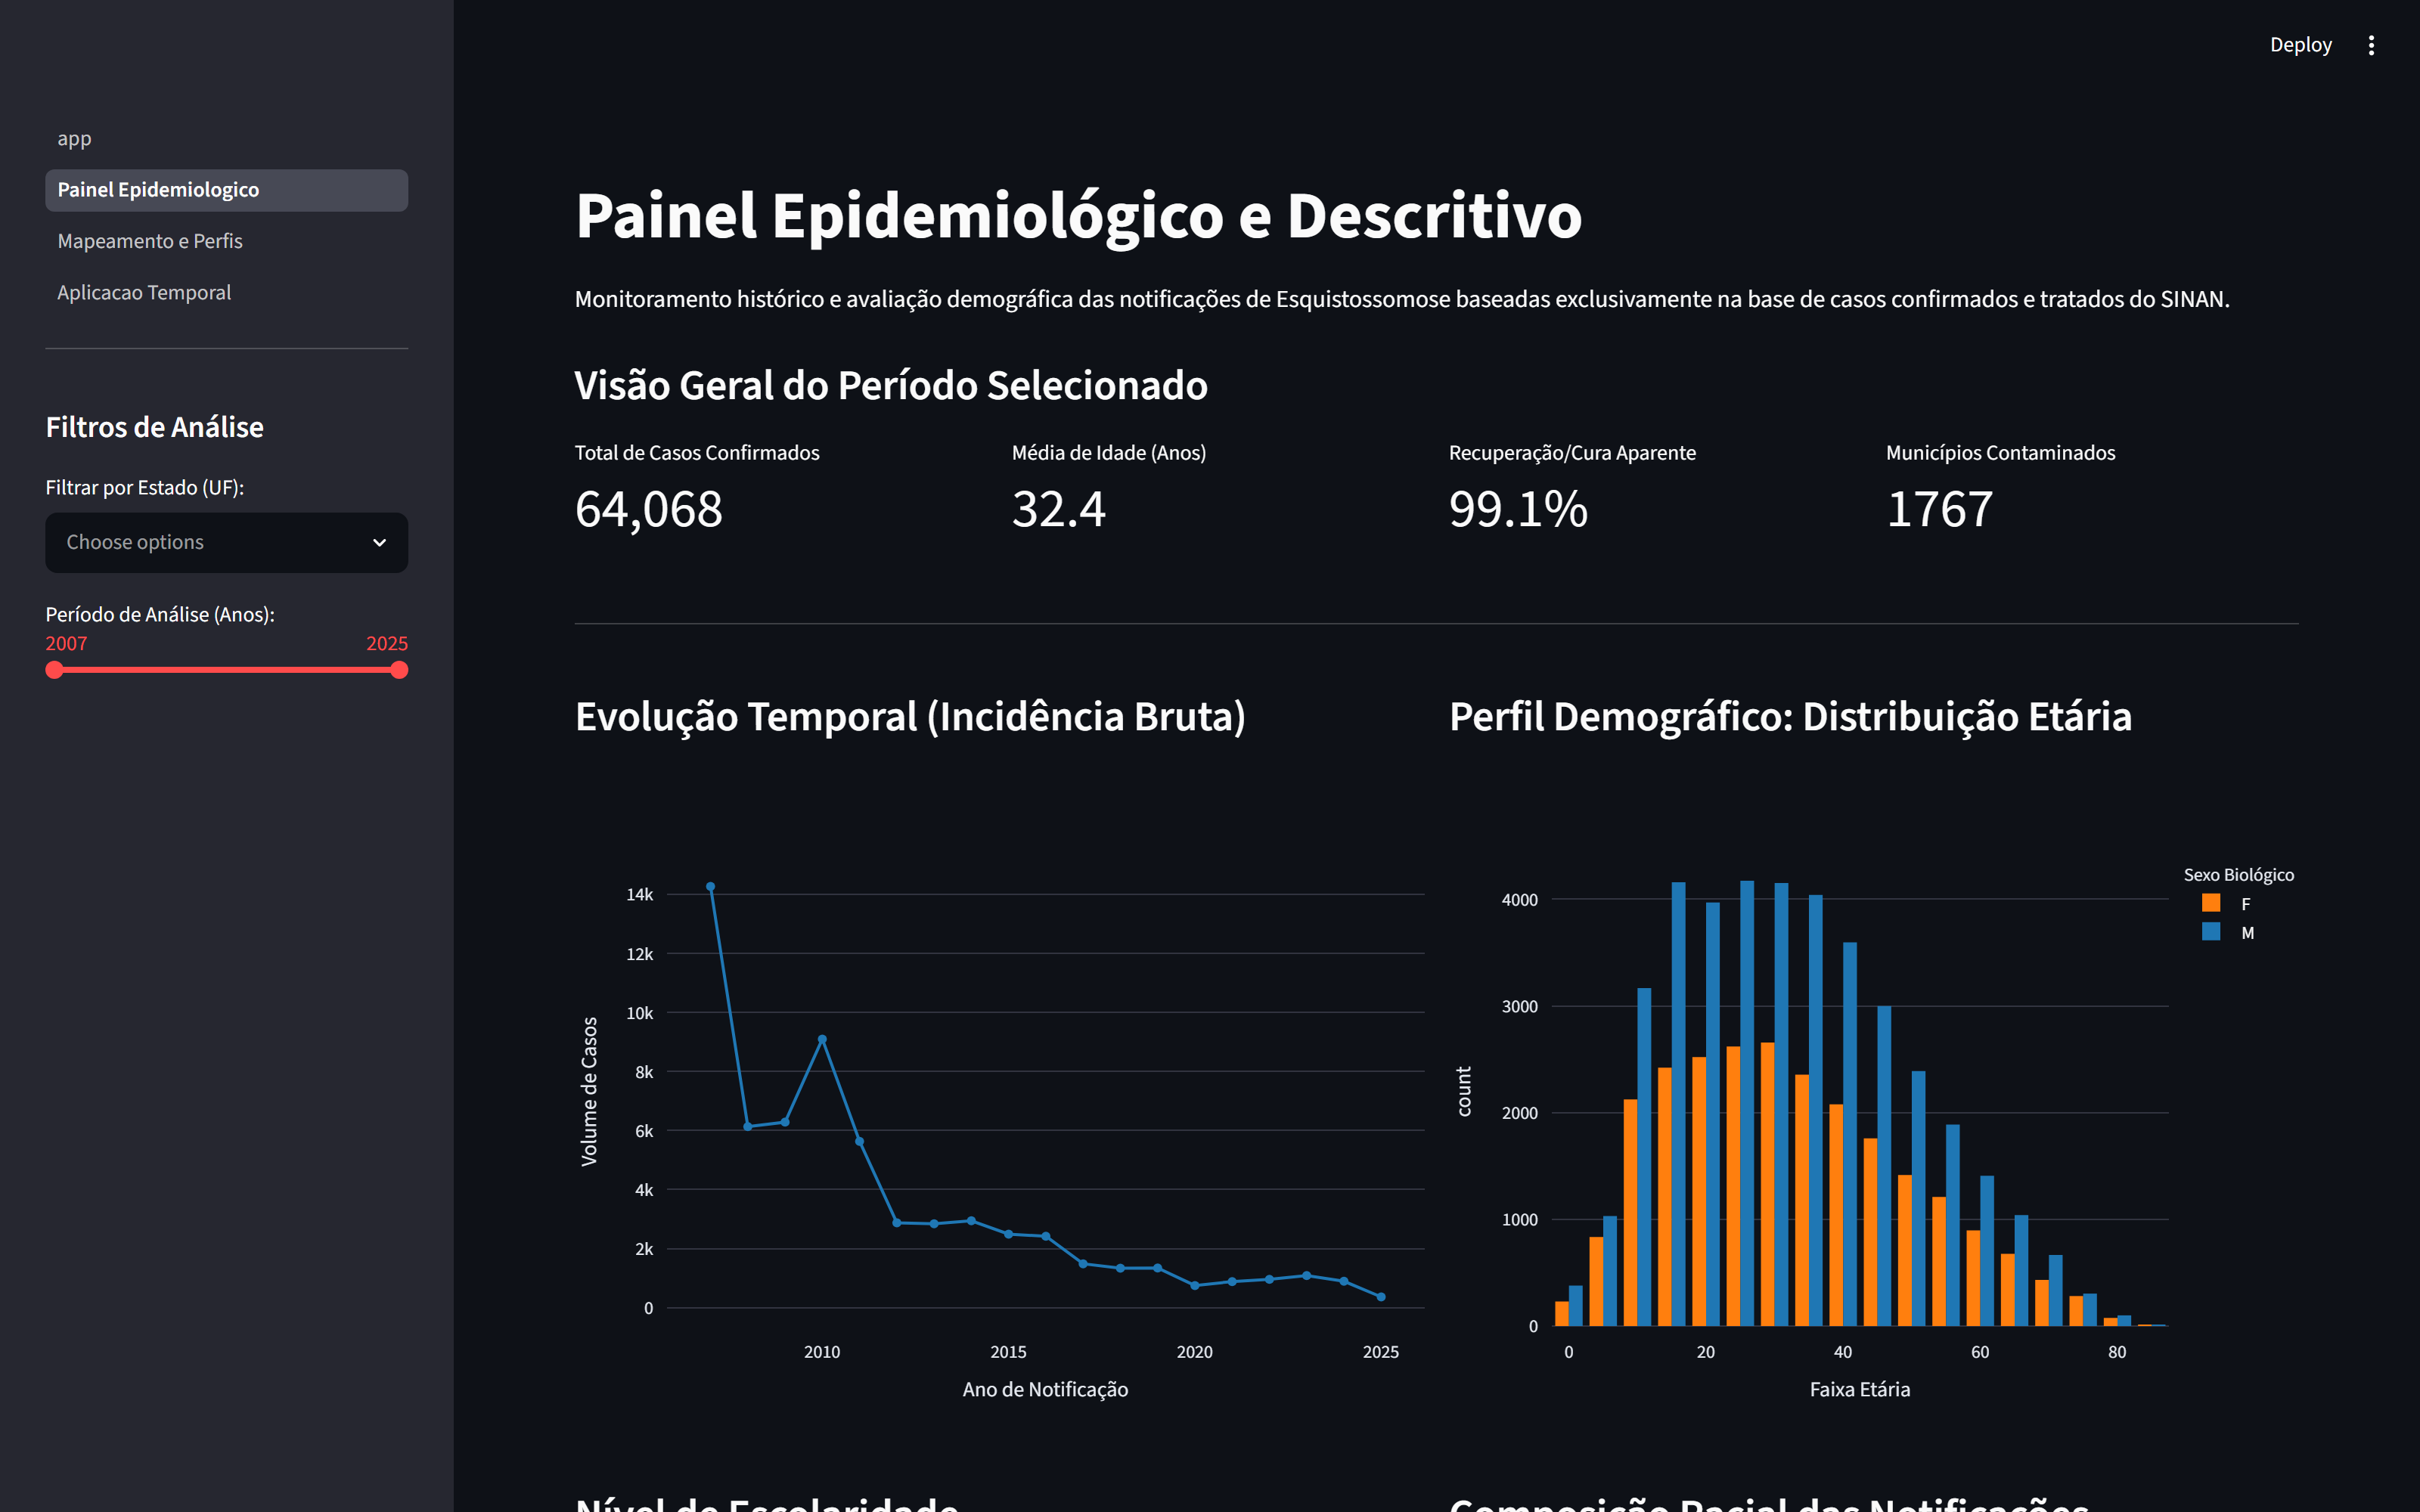
\includegraphics[width=\textwidth]{streamlit_painel.png}
    \caption{Painel Epidemiológico: filtros dinâmicos, métricas e visualizações descritivas do SINAN
    (evolução temporal e distribuição etária por sexo).}
    \label{fig:st_painel}
\end{figure}

\subsection{Mapeamento e Perfis de Risco}

A página de \textbf{Mapeamento e Perfis} (Figura~\ref{fig:st_perfis}) demonstra graficamente o
\emph{Paradoxo do Saneamento} por meio de um gráfico de dispersão (esgoto \textit{versus} incidência)
colorido pelos cinco perfis descobertos pelo K-Means. Complementarmente, a página descreve cada perfil com
cartões de métricas, apresenta a análise das distribuições por perfil (boxplots), oferece uma tabela de
consulta de municípios e um mapa nacional dos focos confirmados.

\begin{figure}[H]
    \centering
    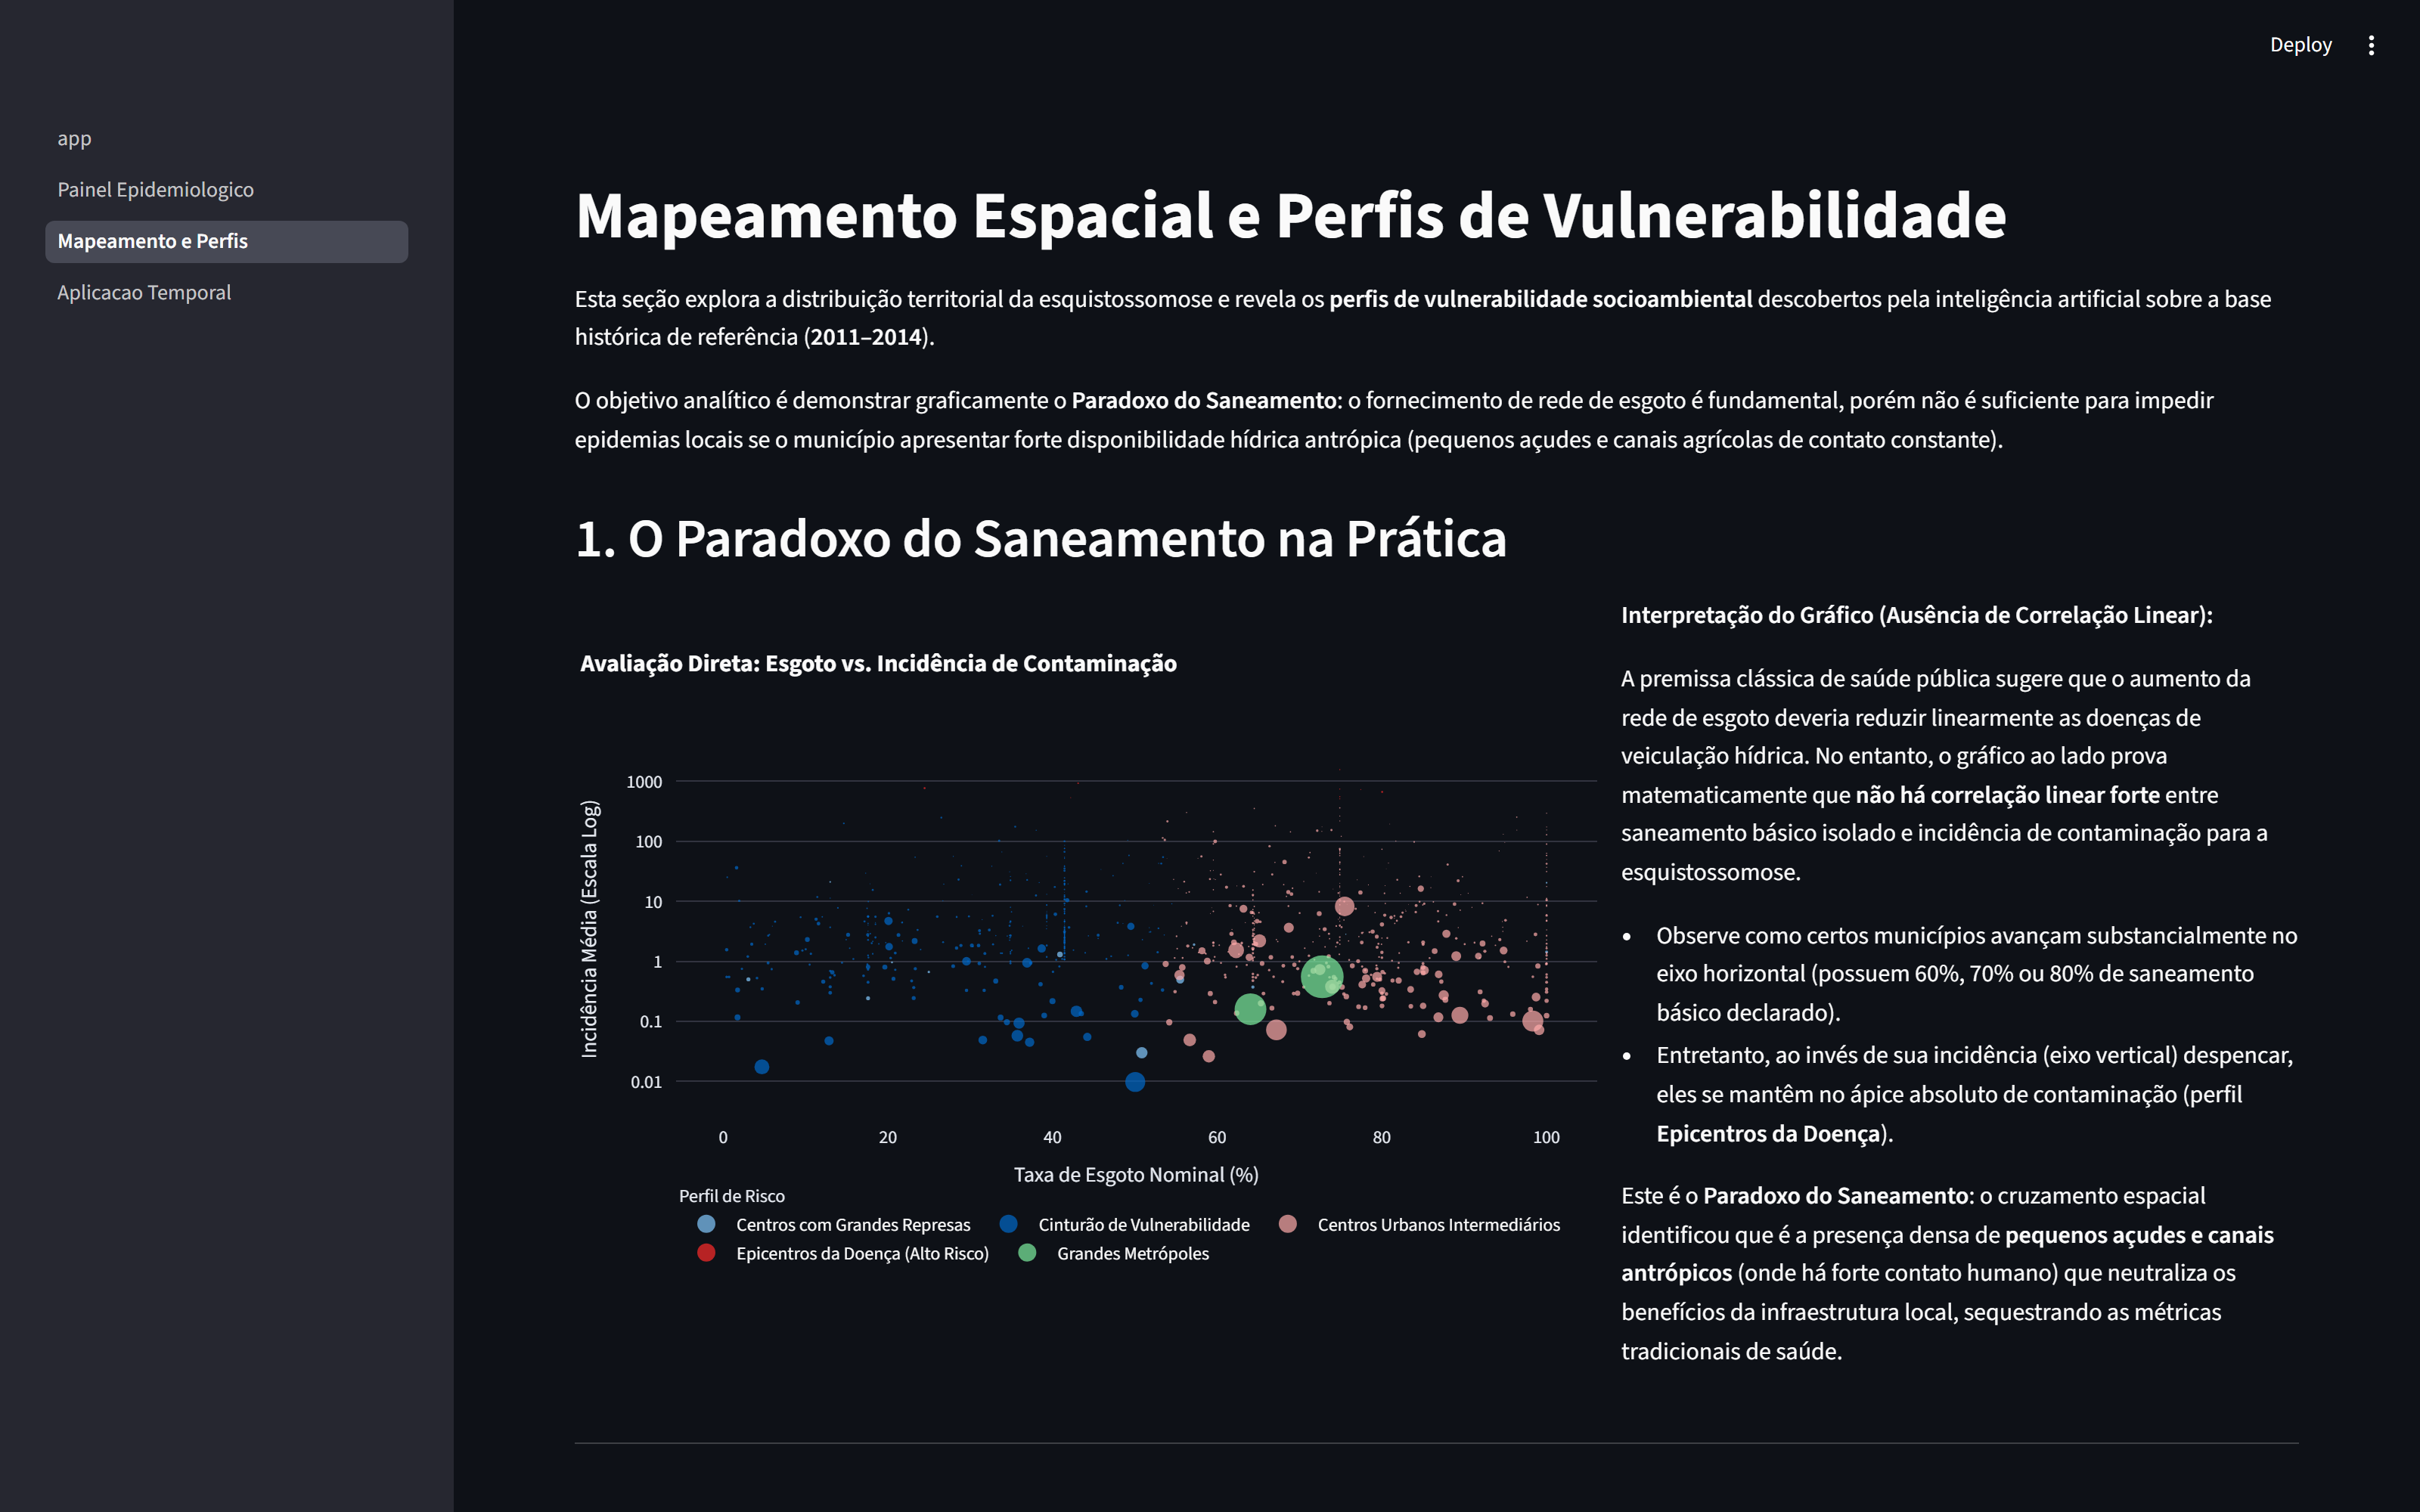
\includegraphics[width=\textwidth]{streamlit_perfis.png}
    \caption{Mapeamento e Perfis: o Paradoxo do Saneamento evidenciado pela ausência de correlação linear
    entre cobertura de esgoto e incidência, com os municípios coloridos pelo perfil de risco.}
    \label{fig:st_perfis}
\end{figure}

\subsection{Aplicação Temporal do Modelo}

A página de \textbf{Aplicação Temporal} (Figura~\ref{fig:st_temporal}) coloca o modelo preventivo em
operação. O usuário seleciona o horizonte (2015--2019 ou 2020--2025) e o sistema aplica o modelo de
referência "às cegas", exibindo: as métricas de desempenho, a matriz de confusão e --- sobretudo --- a
tabela de \textbf{focos emergentes}. Estes são os municípios classificados como alto risco que ainda não
haviam se tornado epicentros: em vez de "erros", são interpretados como candidatos a próximos focos,
constituindo um mapa de vigilância ativa.

\begin{figure}[H]
    \centering
    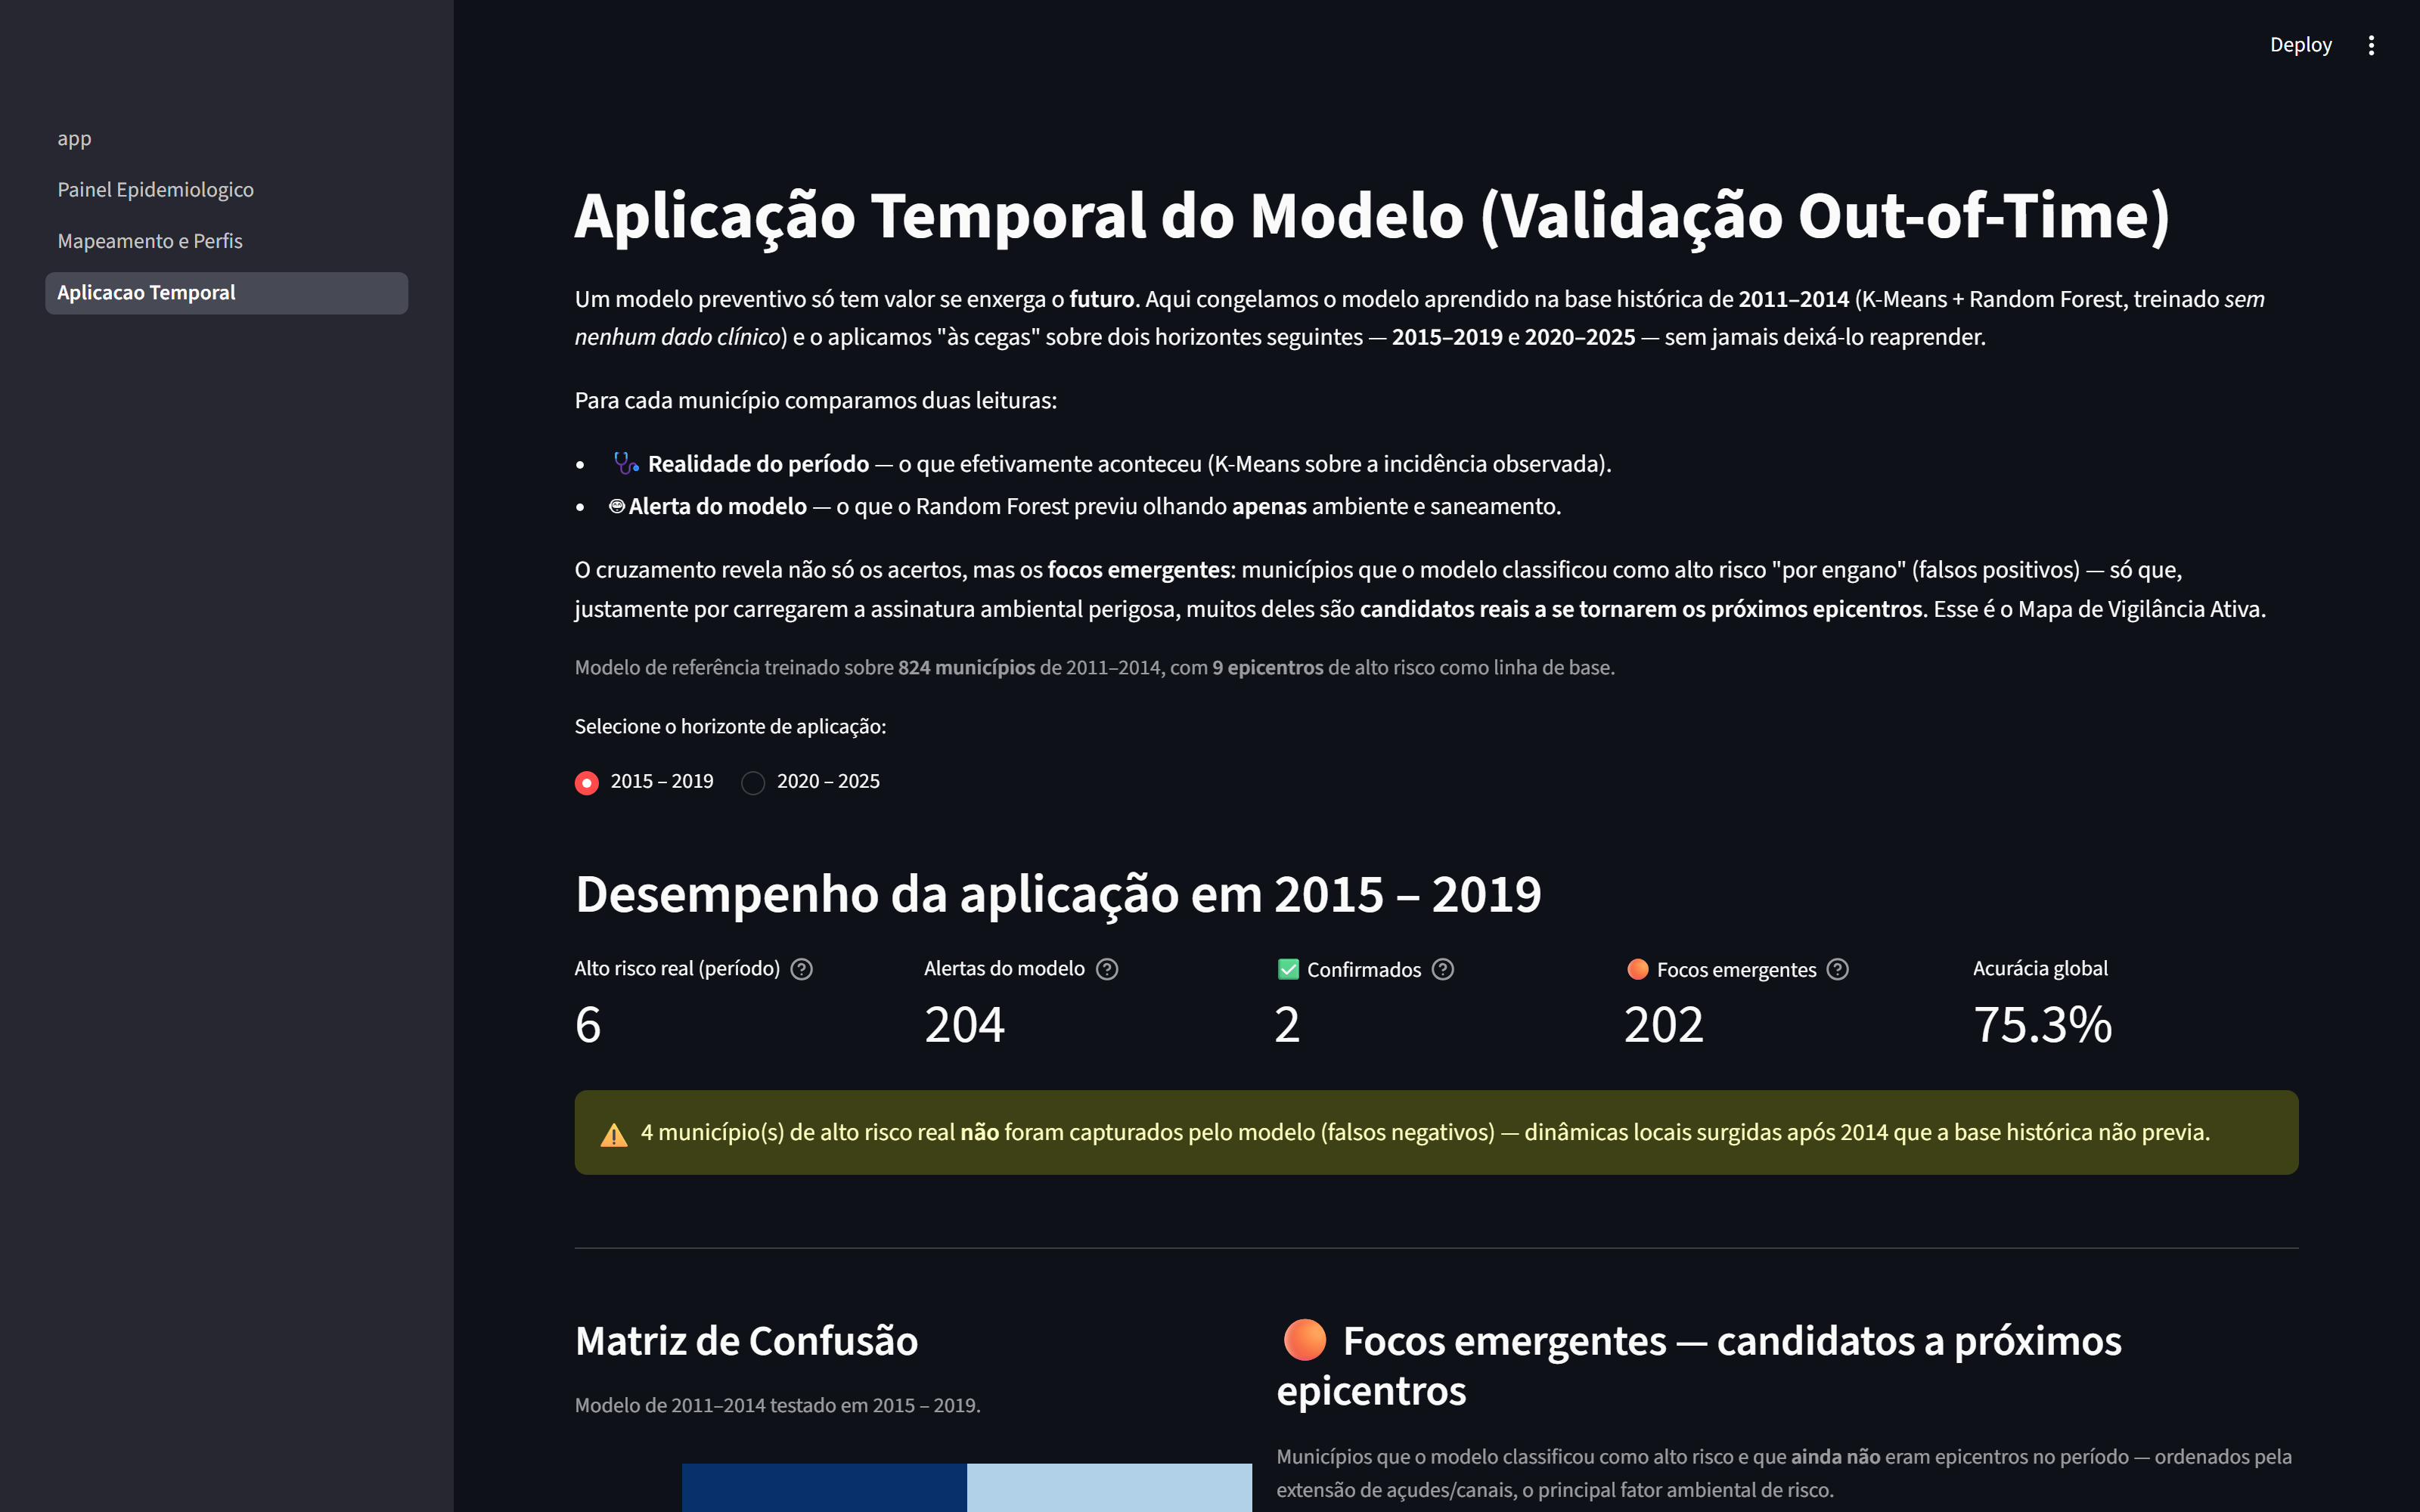
\includegraphics[width=\textwidth]{streamlit_temporal.png}
    \caption{Aplicação Temporal (\textit{Out-of-Time}): o modelo de 2011--2014 aplicado a 2015--2019,
    reproduzindo exatamente os resultados da Fase II (6 epicentros reais, 204 alertas do modelo, 202 focos
    emergentes e 75,3\% de acurácia global).}
    \label{fig:st_temporal}
\end{figure}

\subsection{Aspectos Técnicos e Execução}

A aplicação prioriza desempenho por meio de \textit{cache} agressivo (dados e modelos são carregados e
treinados uma única vez por sessão). As dependências principais são \texttt{streamlit}, \texttt{plotly},
\texttt{scikit-learn}, \texttt{pandas}, \texttt{pyarrow} e \texttt{fastparquet}. A execução local é feita a
partir da raiz do repositório com:

\begin{quote}
\texttt{streamlit run streamlit\_app/app.py}
\end{quote}

% ===================================================================
\part{Considerações Finais}
% ===================================================================

\section{Conclusão Integrada}

O \textit{Projeto Caramujo} percorreu um arco completo de ciência de dados aplicada à saúde pública:
partiu da exploração de uma base clínica limitada, reconheceu suas fronteiras metodológicas e reorientou-se
para uma modelagem socioambiental de maior poder explicativo, culminando em uma ferramenta operacional.

Os principais resultados consolidados foram:

\begin{itemize}
    \item Minas Gerais e Espírito Santo concentram as áreas críticas de transmissão, e fatores locais
    (pequenos açudes e saneamento periférico) exercem maior influência do que as grandes estruturas
    hidrográficas;

    \item a predição de desfechos clínicos individuais mostrou-se limitada pela qualidade e escassez de
    variáveis clínicas, com o XGBoost superando a regressão logística nas classes críticas;

    \item a reformulação socioambiental comprovou matematicamente que a infraestrutura (açudes e
    esgotamento) possui alto sinal preditivo, permitindo prever o risco municipal sem qualquer dado
    clínico;

    \item a validação \textit{Out-of-Time} demonstrou que a assinatura socioambiental de contágio é
    \textbf{estruturalmente atemporal}, ao mesmo tempo em que documentou a expressiva retração histórica da
    doença;

    \item a aplicação em \textit{Streamlit} materializou toda a inteligência do projeto em um sistema
    interativo, reproduzível e coerente com os resultados científicos.
\end{itemize}

\section{Recomendações e Trabalhos Futuros}

\begin{enumerate}
    \item \textbf{Retreino periódico do algoritmo} com a base pós-2020, recalibrando os pontos de corte
    para distinguir a vulnerabilidade latente (risco ambiental) das áreas de surto ativo (risco crônico),
    dado o \textit{concept drift} observado;

    \item inclusão de novas variáveis ambientais e socioeconômicas externas (vulnerabilidade social,
    cobertura de atenção básica) e de coleções hídricas de menor escala (lagoas e áreas de água parada);

    \item aprofundamento da análise geoespacial utilizando Regionais de Saúde como unidade espacial e
    aplicação de métricas de autocorrelação espacial, como o Índice de Moran;

    \item evolução do mapa da aplicação para polígonos municipais reais (GeoJSON/\textit{Pydeck}) e adição
    de filtros mais granulares;

    \item exploração de bases complementares (e-Gestor Atenção Básica) para relacionar infraestrutura de
    saúde com incidência e desfechos;

    \item investigação das alterações epidemiológicas observadas a partir de 2017, buscando identificar os
    fatores associados às mudanças nos padrões registrados.
\end{enumerate}

\end{document}
